\documentclass[12pt]{beamer}

\usepackage{pgfpages} %This is needed for notes presentation!
%\setbeameroption{}

\usepackage{enumerate, amsmath, amssymb,amsthm, amstext,color}
\usepackage[ngerman]{babel}
\usepackage[utf8]{inputenc}   
\usepackage{dsfont}
\usepackage{geometry}
\usepackage{fancyhdr}
\usepackage{tikz}
\usetikzlibrary{plotmarks}
\usetikzlibrary{arrows, positioning}
\usepackage{lmodern}
\usepackage{textcomp}
\usepackage{textpos}

\usepackage{float}
\usepackage{color}
\usepackage{hyperref}
% \usepackage{algorithmicx}
% \usepackage{algpseudocode}
\usepackage{fancybox}
\usepackage{float}
\usepackage{sidecap}
\usepackage[ngerman]{babel}

%\setbeamertamplate[circle]



\newcommand{\lk}{\left}
\newcommand{\rk}{\right}
\newcommand{\rel}{\sqsubseteq}
\newcommand{\rhn}{\mathds{R}^n}
 
\usetheme{Madrid} % Antibes, Berlin, darmstadt, default, Frankfurt; JuanLesPins
%\usetheme{
%	AnnArbor | Antibes | Bergen |
%	Berkeley | Berlin | Boadilla |
%	boxes | CambridgeUS | Copenhagen |
%	Darmstadt | default | Dresden |
%	Frankfurt | Goettingen |Hannover |
%	Ilmenau | JuanLesPins | Luebeck |
%	Madrid | Malmoe | Marburg |
%	Montpellier | PaloAlto | Pittsburgh |
%	Rochester | Singapore | Szeged |
%	Warsaw
%}
\usecolortheme{beaver}
% \usecolortheme{
% 	albatross | beaver | beetle |
% 	crane | default | dolphin |
% 	dove | fly | lily | orchid |
% 	rose |seagull | seahorse |
% 	sidebartab | structure |
% 	whale | wolverine
% }

\useinnertheme{rounded}
% \useinnertheme{
% 	circles | default | inmargin |
% 	rectangles | rounded
% }

\useoutertheme{infolines}
% \useoutertheme{
% 	default | infolines | miniframes |
% 	shadow | sidebar | smoothbars |
% 	smoothtree | split | tree
% }

\usefonttheme{default}
% \usefonttheme{
% 	default | professionalfonts | serif |
% 	structurebold | structureitalicserif |
% 	structuresmallcapsserif
% }

% Seitenzahlen
\setbeamertemplate{footline}[frame number]

\title{Midterm presentation}
\author{The Quadrocopters}
\institute{Technische Universität München}
\date{\today}
% \titlegraphic{\pgfimage[width=1cm,height=1cm]{MA_Web}}
%\logo{\pgfimage[width=1.2cm,height=1.2cm]{MA_Web}}

\beamertemplatenavigationsymbolsempty
% kleine Symbole zur Nvigation wegmachen

\setcounter{MaxMatrixCols}{20}

%\AtBeginSection[]
%{
%	\begin{frame}
%	\frametitle{Overview}
%	\tableofcontents[currentsection]
%	\end{frame}
%}


\begin{document}


\begin{frame}
\maketitle
\end{frame}

\begin{frame}{Overview}
\tableofcontents
\end{frame}

%Der Befehl \include{datei} setzt dann hier die Datei datei.tex ,welche im selben Ordner liegt ein. Diese darf keinen Header enthalten
%\include{datei}

\section{Motivation}
\begin{frame}
	\frametitle{Optimal control problem}
	\begin{block}{}
	  \begin{align*}
		\min_{x,u} J(x,u) \qquad \dot{x} = f(x,u) \\
		x: \textup{state} \\
		u: \textup{control} 
		\end{align*}
	\end{block}
	\vspace{1em}
	 \( \rightarrow \) Additional difficulty: realtime approach
\end{frame}
\begin{frame}{ }
\begin{block}{ }
\centering
\LARGE
 \vspace{1ex}
Model \\
\vspace{1ex}
\end{block}
\end{frame}

\begin{frame}
		\frametitle{Forces and Torques}
		\begin{figure}[p]
			\centering
			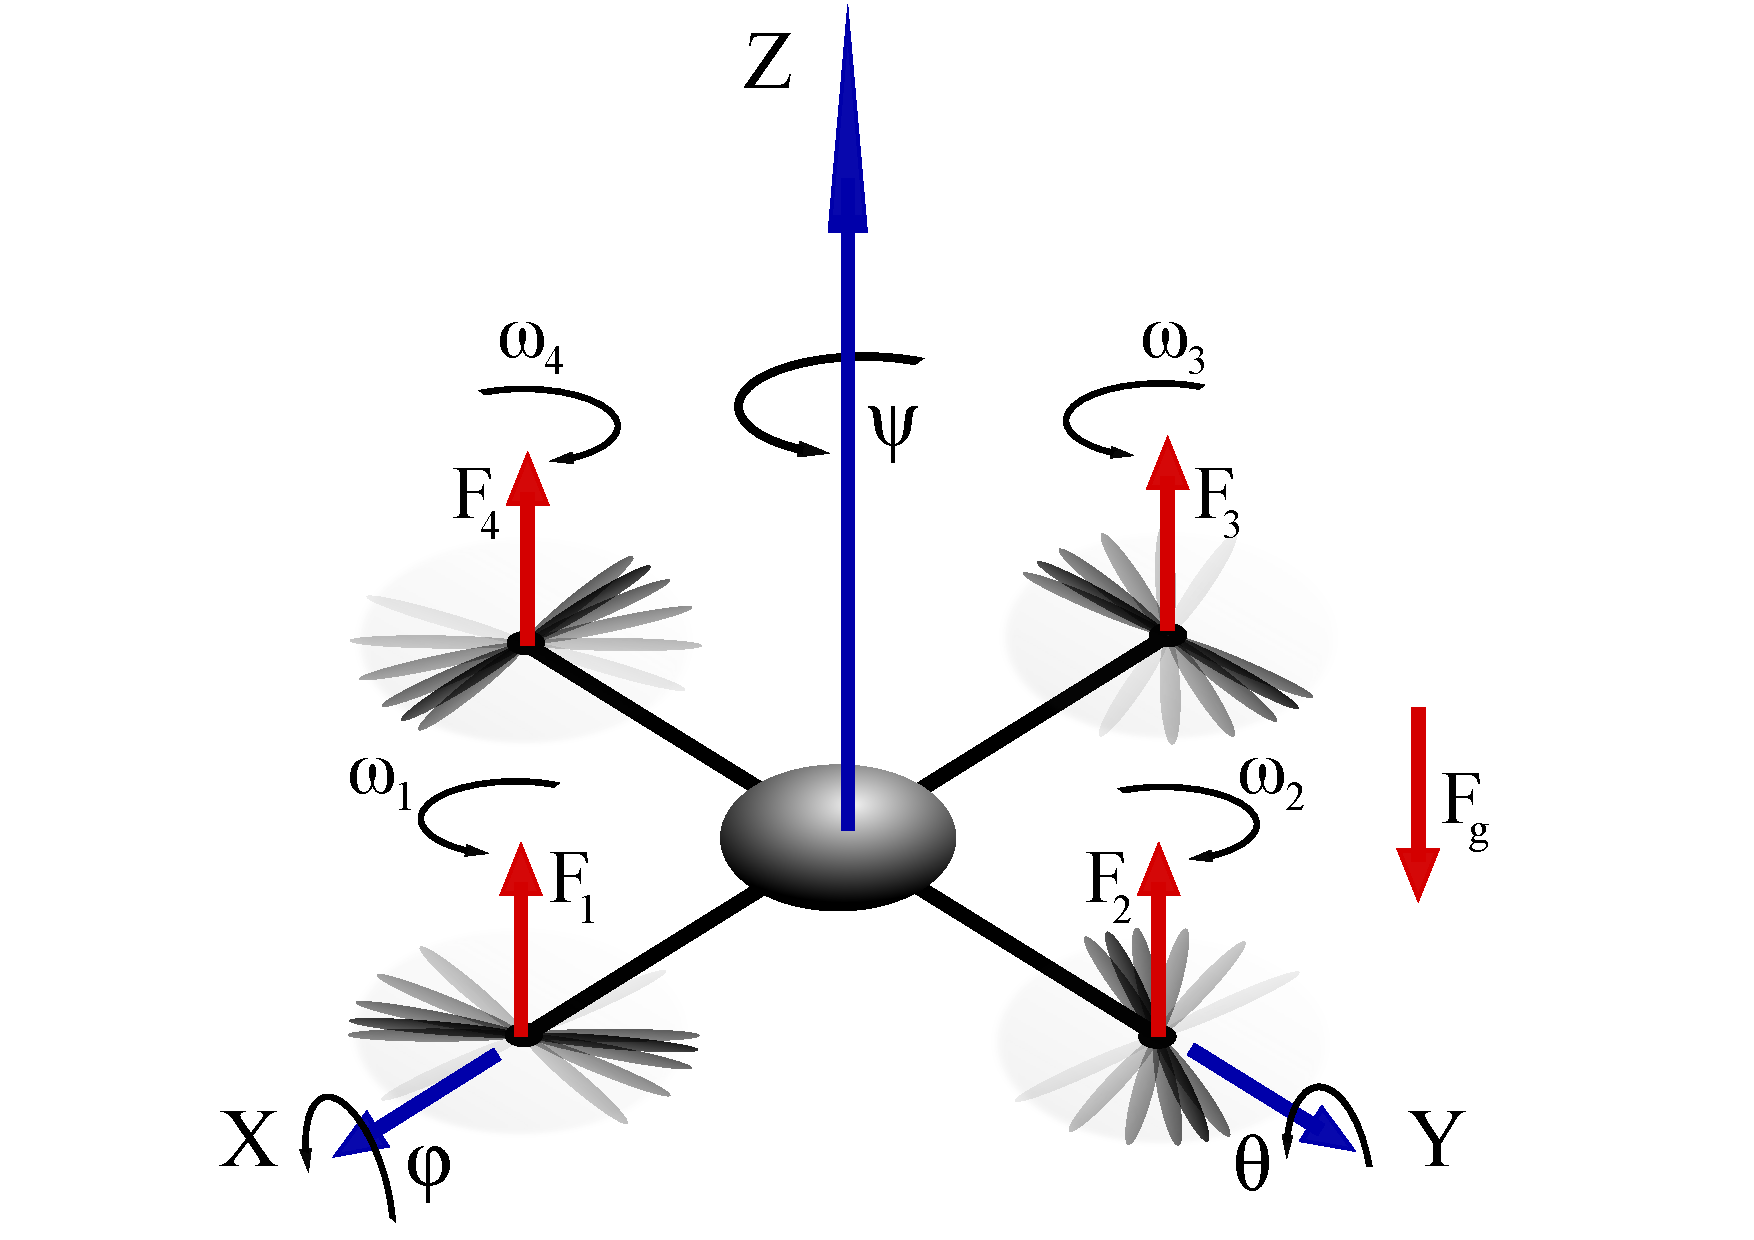
\includegraphics[width=0.8\textwidth]{images/Kraefte.pdf}
			\label{fig:Kraefte}
		\end{figure}
	\end{frame}

	\begin{frame}
		\frametitle{Newton-Euler Equations}
			\begin{columns}[T] % align columns
				\begin{column}{0.70\textwidth}
					Forces \\
					\[ F_{ext} = F_{g} + \sum_{i=1}^{4}{F_{i}} \]
					Torques \\
					\[ \tau_{ext} = \sum_{i=1}^{4}{\tau_{i}}+(\tau_{\varphi}+\tau_{\theta}) \]
				\end{column}
			\hfill
			\begin{column}{.25\textwidth}
				\begin{textblock}{0}(-2,1)
					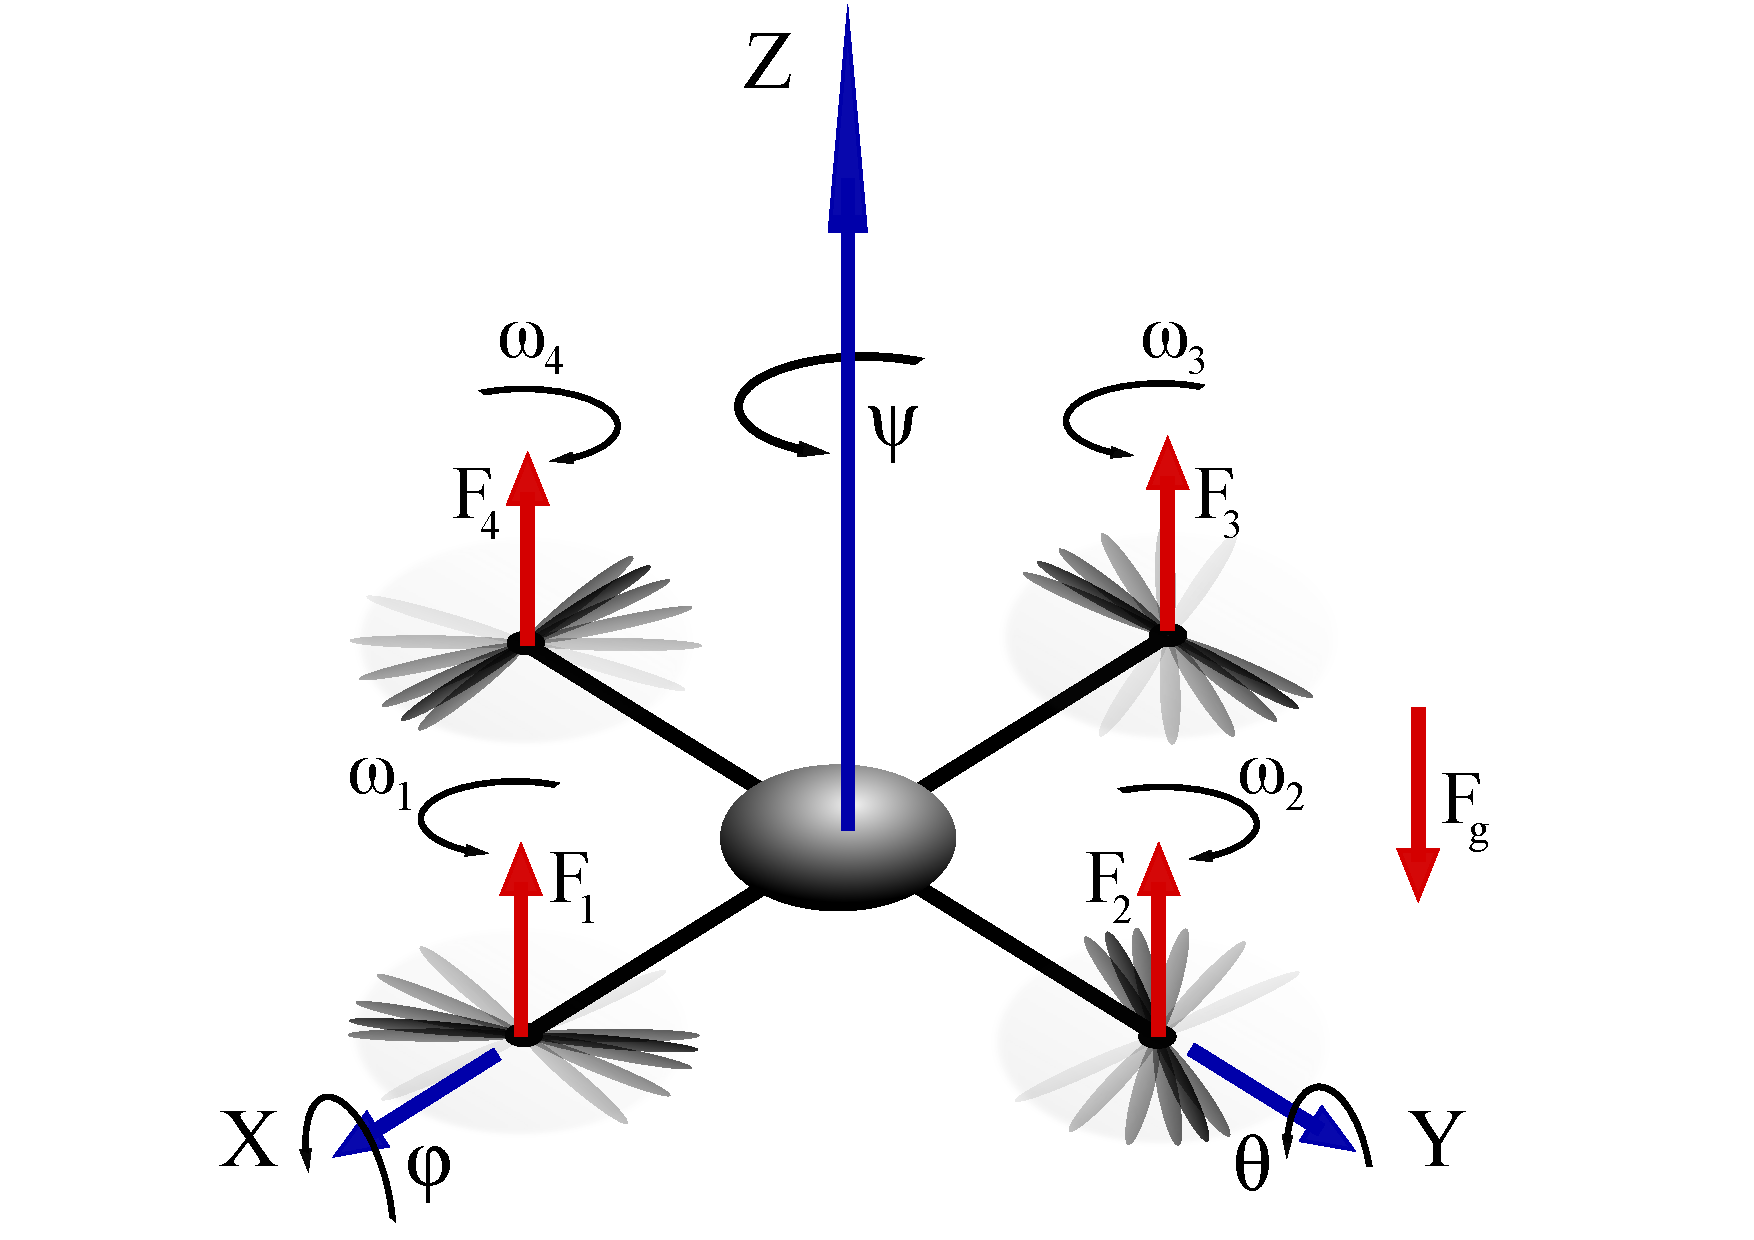
\includegraphics[width=5cm]{images/Kraefte.pdf}
					\label{fig:Kraefte klein}
				\end{textblock}
			\end{column}
		\end{columns}
	\end{frame}
		
	\begin{frame}
		\section{Model}
		\frametitle{Coordinate Systems}
			\begin{figure}[p]
				\centering
				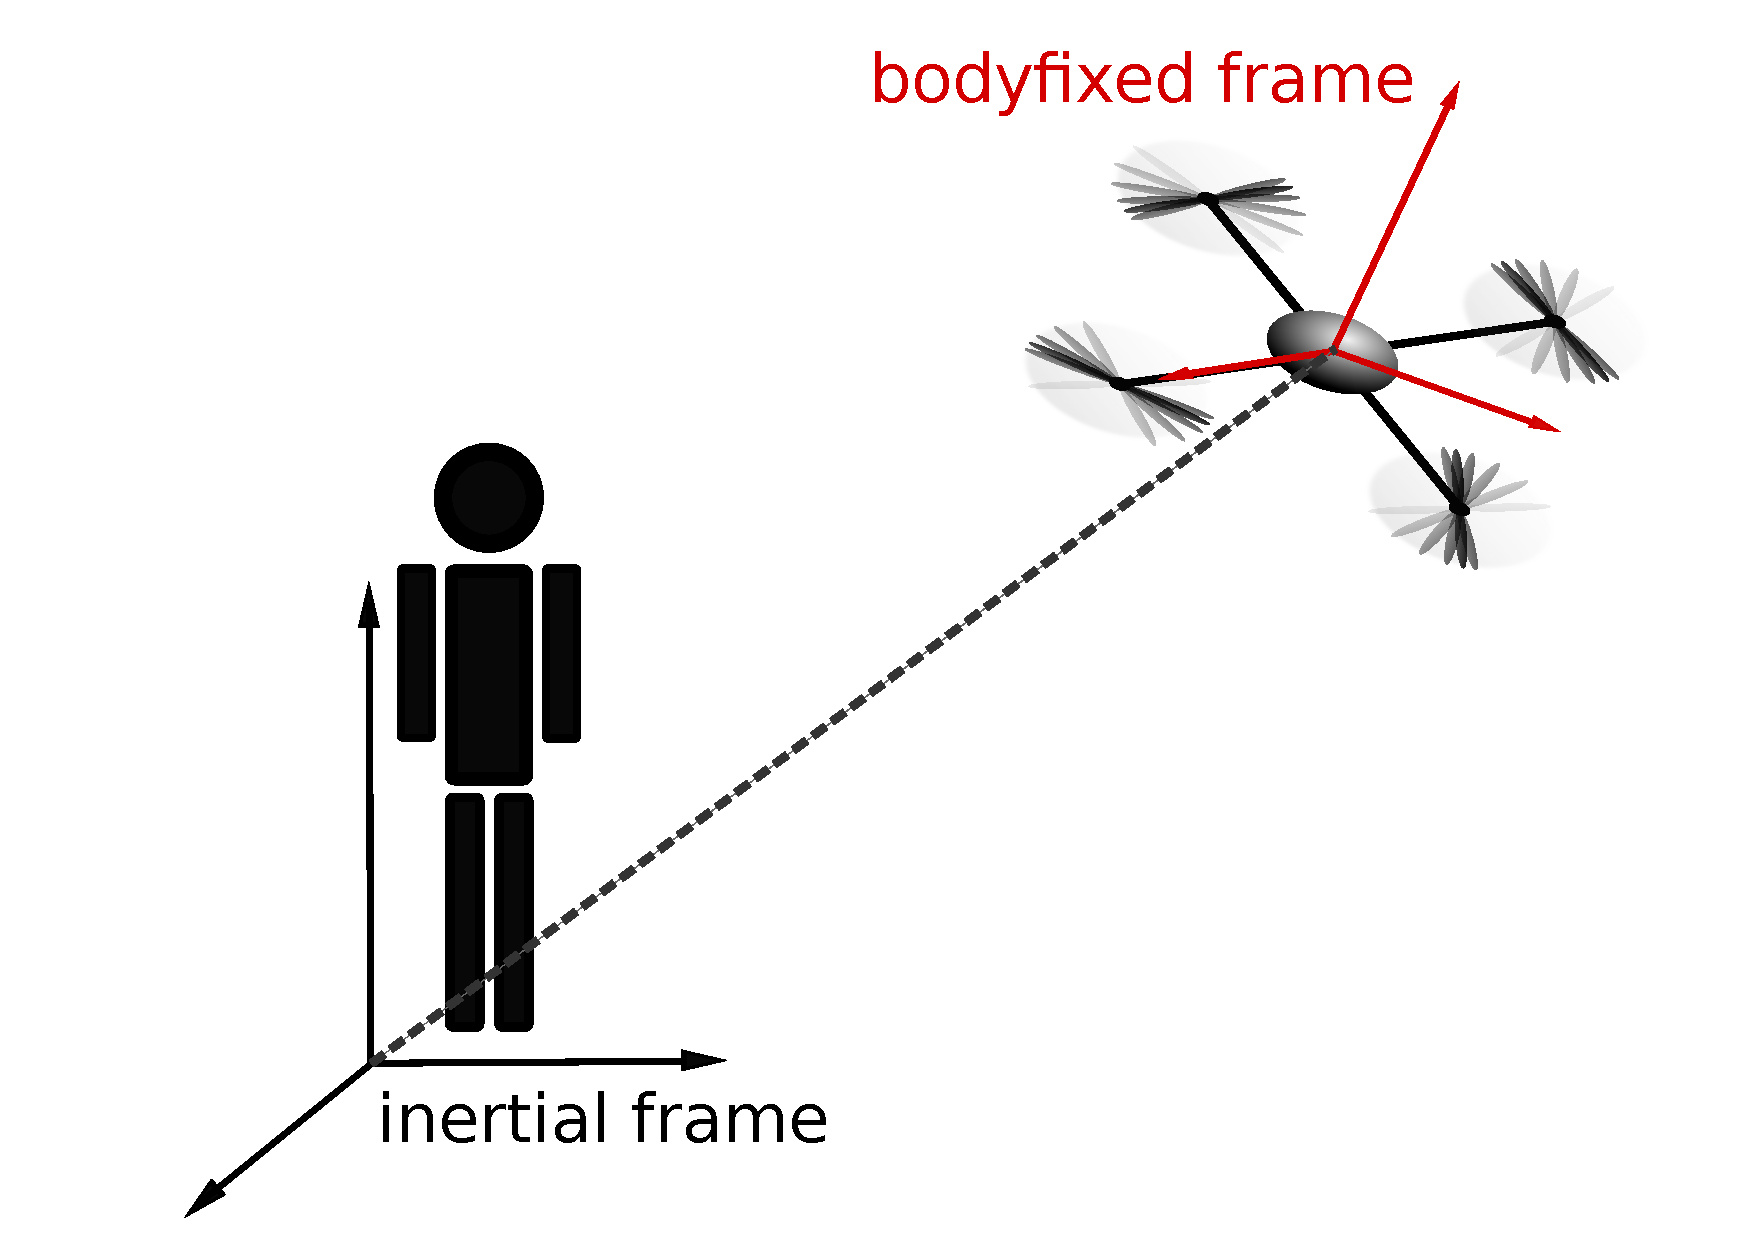
\includegraphics[width=0.8\textwidth]{images/Koordinatensysteme.pdf}
				\label{fig:Koordinatensysteme}
		\end{figure}
	\end{frame}

	
	\begin{frame}
		\frametitle{Quaternions}
		\begin{block}{}
			\[ q = a + \textup{i}b+\textup{j}c+\textup{k}d \qquad a, b, c, d \in \mathbb{R} \]
			\vspace{.1ex}
			\end{block}
			
			\vspace{1ex}
			\onslide<2-> representing rotation \( \Leftrightarrow \) \( \Vert q \Vert = 1 \) \\
			\vspace{1ex}			
			\onslide<3-> advantage \(\rightarrow\) no singularities \\
			\vspace{1ex}
			\onslide<4-> problem \(\rightarrow\) \( \Vert q \Vert = 1 \) additional constraint
	\end{frame}
	
	\begin{frame}
		\frametitle{Dynamics}
		Equations representing dynamics...
		\[ T(x, u) = M \cdot \begin{pmatrix} \dot{x}_{8} \\ \vdots \\ \dot{x}_{13} \end{pmatrix} + \Theta(x) \]
		\onslide<2->
		...expressed as system of differential equations:
		\[ \frac{\textup{d}}{\textup{d}t} 
			\begin{pmatrix}
						  x_{1} \\ \vdots \\ x_{7} \\ x_{8} \\ \vdots \\ x_{13}
			\end{pmatrix}
			=
			\begin{pmatrix}
							\dot{x}_{1} \\ \vdots \\ \dot{x}_{7} \\ M^{-1}(T(x,u)-\Theta(x))
			\end{pmatrix}
		\]
	\end{frame}
	
	\begin{frame}
		\frametitle{Prospect}
			Refinement of the model \\
			\vspace{1ex}
			\(\rightarrow\) wind \\
			\vspace{1ex}
			\(\rightarrow\) aerodynamical forces \\
	\end{frame}

%Der Befehl \include{datei} setzt dann hier die Datei datei.tex ,welche im selben Ordner liegt ein. Diese darf keinen Header enthalten
%\include{datei}
\begin{frame}{ }
\begin{block}{ }
\centering
\LARGE
 \vspace{1ex}
Realtime Optimization Approach\\
\vspace{1ex}
\end{block}
\end{frame}
%\documentclass{beamer}
%
%\usepackage{pgfpages} %This is needed for notes presentation!
%%\setbeameroption{}
%
%\usepackage{enumerate, amsmath, amssymb,amsthm, amstext,color}
%\usepackage[ngerman]{babel}
%\usepackage[utf8]{inputenc}   
%\usepackage{dsfont}
%\usepackage{geometry}
%\usepackage{fancyhdr}
%\usepackage{tikz}
%\usetikzlibrary{plotmarks}
%\usetikzlibrary{arrows, positioning}
%
%\usepackage{float}
%\usepackage{color}
%\usepackage{hyperref}
%% \usepackage{algorithmicx}
%% \usepackage{algpseudocode}
%\usepackage{fancybox}
%\usepackage{float}
%\usepackage{sidecap}
%\usepackage[ngerman]{babel}
%
%
%\newcommand{\lk}{\left}
%\newcommand{\rk}{\right}
%\newcommand{\rel}{\sqsubseteq}
%\newcommand{\rhn}{\mathds{R}^n}
% 
%  \usetheme{Berlin}
%%\usetheme{
%%	AnnArbor | Antibes | Bergen |
%%	Berkeley | Berlin | Boadilla |
%%	boxes | CambridgeUS | Copenhagen |
%%	Darmstadt | default | Dresden |
%%	Frankfurt | Goettingen |Hannover |
%%	Ilmenau | JuanLesPins | Luebeck |
%%	Madrid | Malmoe | Marburg |
%%	Montpellier | PaloAlto | Pittsburgh |
%%	Rochester | Singapore | Szeged |
%%	Warsaw
%%}
%\usecolortheme{beaver}
%% \usecolortheme{
%% 	albatross | beaver | beetle |
%% 	crane | default | dolphin |
%% 	dove | fly | lily | orchid |
%% 	rose |seagull | seahorse |
%% 	sidebartab | structure |
%% 	whale | wolverine
%% }
%
%\useinnertheme{rounded}
%% \useinnertheme{
%% 	circles | default | inmargin |
%% 	rectangles | rounded
%% }
%
%\useoutertheme{infolines}
%% \useoutertheme{
%% 	default | infolines | miniframes |
%% 	shadow | sidebar | smoothbars |
%% 	smoothtree | split | tree
%% }
%
%\usefonttheme{default}
%% \usefonttheme{
%% 	default | professionalfonts | serif |
%% 	structurebold | structureitalicserif |
%% 	structuresmallcapsserif
%% }
%
%% Seitenzahlen
%\setbeamertemplate{footline}[frame number]
%
%\title{Mid-term presentation}
%\author{The Quadrocopters}
%\institute{Technische Universität München}
%\date{\today}
%% \titlegraphic{\pgfimage[width=1cm,height=1cm]{MA_Web}}
%%\logo{\pgfimage[width=1.2cm,height=1.2cm]{MA_Web}}
%
%
%%\AtBeginSection[]{
%%	\frame{
%%	\frametitle{\"Ubersicht}
%%	\tableofcontents[current, currentSection]}
%%
%%}
%
%\setcounter{MaxMatrixCols}{20}
%
%\begin{document}

\definecolor{green}{RGB}{0,190,45}
\definecolor{green2}{RGB}{0,150,45}
\definecolor{red}{RGB}{190,0,0}
\definecolor{blue}{RGB}{0,0,190}

%\begin{frame}
%\maketitle
%\end{frame}
%
%\begin{frame}
%\tableofcontents
%\end{frame}

\section{Realtime Optimization Approach}
\begin{frame}{Setting}

\begin{figure}
\begin{tikzpicture}[scale=1.2]

%Draw bounding box
\draw (-2.75,-1.75) rectangle (3.75,3.25);

%Draw time line
\draw[ thick, ->] (-2.5,0) -- (2,0) node[anchor=west] {time};
\foreach  \t in  {-2, -1, +1}
	\draw[thick]  (\t cm, 1pt)  -- (\t cm, -1pt) node[anchor=north] {\footnotesize $t \t $ };
\draw[thick]  (0cm , 1pt)  -- (0 cm, -1pt) node[anchor=north] {\footnotesize $t$ };

%draw known controls
\draw<2-> (2,1) node[anchor=west] {control};
\draw<2->[->,green2] (-2.5, 0.8) -- (-2,0.8) ;
\draw<2->[->,green2] (-2, 1.2) -- (-1,1.2) ;
\draw<2->[->,green2] (-1, 0.9) -- (0,0.9) ;
\draw<4->[->,red,thick] (0, 1.1) -- (1,1.1) ;

%Draw actual time
\draw[dashed] (-.65,3) -- (-.65,-1) node[anchor=north] {$t_{act}$};

%Draw exact states
\draw<2-> (2,2) node[anchor=west] {state};
\draw<2->[green2, fill=green2] (-2, 2.2) circle (1pt) node[anchor=north]{\footnotesize $x_{t-2}$};
\draw<2->[green2, fill=green2] (-1, 1.9) circle (1pt) node[anchor=north]{\footnotesize $x_{t-1}$};
\draw<3->[red, fill=red] (0,2.1) circle (1pt) node[anchor=north]{\footnotesize $x_{t}$};
\end{tikzpicture}
\end{figure}
\end{frame}

\begin{frame}{Discrete Problem}
\begin{block}{}
%\begin{align*}
\[  \min_{x, u} \sum_{i=t}^{t+N} J_{i}(x_{i},u_{i}) \qquad  
  \text{s.t.} \quad 
  h_i (x_i ,u_i ) = 0 \quad  i = t, ... , t+N  \]
%\end{align*}
\end{block}
\vspace{2em}
\begin{tabular}{l l}
  $J_i(x_i, u_i)$ &  discretized goal function 
%  \vspace{1ex} \\
%$x_t - s_t = 0$ & expected state $=$ real state
  \vspace{1ex} \\
$h_i (x_i ,u_i )$ & equality constraints at time $i$ 
\end{tabular}
\end{frame}

\definecolor{green}{RGB}{0,190,0}
\definecolor{red}{RGB}{190,0,0}
\definecolor{gray}{RGB}{35,10,10}

\begin{frame}
\centering

\begin{tikzpicture}[node distance=1.3cm, font=\Large,
					neutral/.style ={
					%shape
					rectangle, minimum size=9mm, minimum width=3cm, rounded corners=2mm,
					%rest
					very thick, draw=gray!30,
					top color=gray!5, bottom color=gray!20},
					aktiv/.style ={
					rectangle, minimum size=9mm, minimum width=3cm, rounded corners=2mm,
					very thick, draw=red,
					top color=red!20, bottom color=red!70},
					fertig/.style ={
					rectangle, minimum size=9mm, minimum width=3cm, rounded corners=2mm,
					very thick, draw=green!70,
					top color=green!20, bottom color=green!70}]

%\draw (-1,0) rectangle (10,-5);
%\draw (-1,0) rectangle (10,-5);
\draw  
	node[neutral, minimum width=10.5cm] (r) {Results}
	node[aktiv, above=of r.east, anchor=east] (f) {Realtime}
	node[aktiv, above=of f.east, anchor=east] (e) {Riccati}
	node[aktiv, above=of e.east, anchor=east] (g) {SQP}
	node[fertig, above=of r.west, minimum width=7cm, anchor=west] (d) {Problemformulation}
	node[fertig, above=of d.west, anchor=west] (b) {Quaternions} 
	node[fertig, above=of d.east, anchor=east] (c) {Discretization}
	node[fertig, minimum width=3.145cm, above=of b.west, anchor=west] (a) {Model}
	;
	
	\draw[very thick,->] (a) -- +(0,-0.8);
	\draw[very thick,->] (b) -- +(0,-0.8);
	\draw[very thick,->] (c) -- +(0,-0.8);
	\draw[very thick,->] (d) -- +(0,-0.8);
	\draw[very thick,->] (e) -- +(0,-0.8);
	\draw[very thick,->] (f) -- +(0,-0.8);
	\draw[very thick,->] (g) -- +(0,-0.8);
	
	\end{tikzpicture}

\end{frame}

\begin{frame}{The Lagrangian}
\begin{block}{ }
%\begin{align*}
%\begin{array}{c}
\[  L(y) =   \sum\limits_{i=t}^{t+N} J_{i}(x_{i},u_{i})
%  + \lambda_{t}^{T}(x_{t} - s_{t}) 
  + \sum\limits_{i=t}^{t+N} \lambda_{i}^{T} h_i (x_i ,u_i ) \]
%  \end{array}
%\end{align*}
%\vspace{.1ex}
\end{block}
\begin{gather*}
	y := (\lambda,x,u) \\
	\vspace{1ex}
	y^* \text{ optimal} \quad \Leftrightarrow \quad \nabla_{y} L(y^*)  = 0
\end{gather*}

\end{frame}

%\begin{frame}
%	\frametitle{SQP-Formulation}
%	
%	\begin{block}{}
%		\centering
%			\parbox{7cm}{\( \min \limits_{x,u} J(x,u) \qquad \text{s.t.} \qquad h(x,u) = 0 \)	}
%\end{block}
%	
%	\uncover<2>{
%		\center{
%		reformulation as SQP-Problem \\
%		\vspace{1ex}
%		\(\Downarrow\)
%		\vspace{1em}
%		}
%		
%		
%		\begin{block}{}
%		\centering
%			\parbox{7cm}{\[ \min \limits_{s} \nabla J(x,u)^T s + \frac{1}{2}s^T \nabla^2 J(x,u)s \]
%			 \[ \text{s.t.} \quad  h(x,u) + \nabla h(x,u)^Ts = 0 \]	}
%	\end{block}
%	}
%	
%\end{frame}

\begin{frame}{The SQP Method}
Find $y^*$:
\begin{block}{ }
%\begin{gather*}
\[ y_{1} = y_{0} + s \]
\[\min_{s}  \frac{1}{2} s^T \nabla^2 L(y_0) s + \nabla L(y_0)^T s \]
%\end{gather*} \vspace{.1ex}
\end{block}
%\onslide<2->
%\vspace{1ex}
%Special case: \\
%\vspace{1ex}
%\begin{tabular}{l l}
%$ A_{k} = H(y_k)$ & approximated Hessian $\nabla^{2}_{y_k} L(y_k)$ \vspace{1ex} \\
%$\alpha_k = 1$ & 
%\end{tabular}
\hfill
\centering
\definecolor{green}{RGB}{0,190,0}
\definecolor{red}{RGB}{190,0,0}
\definecolor{gray}{RGB}{35,10,10}

\begin{tikzpicture}[scale = 1.4,domain=-2:3.7]
	\def \point {1};
	
	%Gitter zeichnen
	\draw[very thin,color=gray!30] (-2.1,-1.1) grid (5.2,1.2);
	%Achsen zeichnen
	\draw[->] (-2.2,0) -- (5.2,0) node[right] {$y$};
	\draw[->] (0,-1.2) -- (0,1.2) node[above] {};
	%Funktion zeichnen
	\draw[thick, color=blue] plot (\x, {0.07*(\x)^3 -  0.7*(\x) }) node[right] {$L(y)$};
	\draw[thick, color=red] plot (\x + \point, {(0.5*(0.42*(\point))*(\x)^2 + (0.21*(\point)^2-0.7)*(\x))  +(0.07*(\point)^3 -  0.7*(\point) )} );
%	\draw[thick, color=green] plot (\x , {((0.21*(\point)^2-0.7) + (0.42*(\point))*(\x)) });
%	\draw[thick, mark=x] plot (\point , {(0.07*(\point)^3 -  0.7*(\point) )}) ;
	\draw[thick, dashed] (\point ,0) node[above] {$y_0$} -- (\point,{(0.07*(\point)^3 -  0.7*(\point) )}) ;
%	\draw[thick, decorate, decoration={brace,amplitude=6pt}] (0,0) -- ({- (0.21*(\point)^2-0.7)/(0.42*(\point))},0) node[midway, above,yshift=3pt,]{$s_k$};
	\draw[thick, mark=*, mark size=1pt] plot (\point , {(0.07*(\point)^3 -  0.7*(\point) )}) ;
	\draw[thick] plot ({\point - (0.21*(\point)^2-0.7)/(0.42*(\point))} , 0) node[above] {$y_{1}$};
	\draw[thick, dashed] ({\point - (0.21*(\point)^2-0.7)/(0.42*(\point))} , 0) --++ (0,-0.93);
	\draw[thick, mark=*, mark size=1pt] plot ({\point - (0.21*(\point)^2-0.7)/(0.42*(\point))},-0.93);
	
	%\draw[thick, color=black] plot (\x, {0.21*(\x)^2 -  0.7 });
	\end{tikzpicture}
	
%	\begin{tikzpicture}[domain=-2:4]
%	\def \point {1};
%	
%	%Gitter zeichnen
%	\draw[very thin,color=gray!30] (-2.1,-1.1) grid (5.2,2.2);
%	%Achsen zeichnen
%	\draw[->] (-2.2,0) -- (5.2,0) node[right] {$y$};
%	\draw[->] (0,-1.2) -- (0,2.2) node[above] {$L(y)$};
%	%Funktion zeichnen
%	\draw[thick, color=blue] plot (\x, {0.07*(\x)^3 -  0.7*(\x) });
%	\draw[thick, color=red] plot (\x + \point, {(0.5*(0.42*(\point))*(\x)^2 + (0.21*(\point)^2-0.7)*(\x))  +(0.07*(\point)^3 -  0.7*(\point) )} );
%	\draw[thick, color=green] plot (\x , {((0.21*(\point)^2-0.7) + (0.42*(\point))*(\x)) });
%	\draw[thick, mark=x] plot (\point , {(0.07*(\point)^3 -  0.7*(\point) )}) ;
%	\draw[thick, decorate, decoration={brace,amplitude=6pt}] (0,0) -- ({- (0.21*(\point)^2-0.7)/(0.42*(\point))},0) node[midway, above,yshift=3pt,]{$s_k$};
%	
%%	\draw[thick, mark=x] plot ({\point - (0.21*(\point)^2-0.7)/(0.42*(\point))} , 0) node[below] {$y_{k+1}$};
%	
%	%\draw[thick, color=black] plot (\x, {0.21*(\x)^2 -  0.7 });
%	\end{tikzpicture}

\end{frame}

\begin{frame}{Quasi Newton-Method}
Find $s$ with:
\begin{block}{}
%\begin{gather*}
\[ \nabla L(y_{0}) + \nabla^2 L(y_0) s = 0 \]
%\end{gather*} \vspace{.1ex}
\end{block} 
\vspace{1em}
Approximate $\nabla^2 L(y_0)$ and solve:
\begin{block}{}
%\begin{gather*}
\[ H(y_0) s = -\nabla L(y_{0}) \]
%\end{gather*} \vspace{.1ex}
\end{block} 
%1 iteration per timestep:
%\begin{block}{ }
%\begin{gather*}
%y_{t+1} = y_1 = y_0 + \Delta y_0 \\
%\end{gather*}
%\end{block}
\end{frame}

\begin{frame}{Riccati Recursion}

\begin{figure}
\begin{tikzpicture}
%Draw bounding box
\draw[black] (-1.5,-4.5) rectangle (3.5,0.5);
\draw[white,fill=white] (-1.4,0.6) rectangle (3.4,-4.6);
%Schrift einfügen
\draw (1,-5.2) node {\large $H(y_0)$}
		(4.2,-5.2) node {\large $s$}
		(5.7,-5.2) node {\large $-\nabla L(y_{0})$};

\draw[black] (3.9,0.5) rectangle (4.5,-4.5);
\draw[white,fill=white] (4,0.6) rectangle (4.4,-4.6);

\draw[black] (5.4,0.5) rectangle (6,-4.5);
\draw[white,fill=white] (5.5,0.6) rectangle (5.9,-4.6);

\draw[thick, -] (4.7,-1.85) -- (5.2,-1.85);
\draw[thick, -] (4.7,-2.15) -- (5.2,-2.15);

\draw[blue,fill=blue] (-1,0.4) rectangle (-0.6, 0);
\draw[blue,fill=blue] (-1.4,0) rectangle (-1, -0.4);
\draw[blue,fill=blue] (-0.4,-0.6) rectangle (0.4, -1.4);
\draw[blue,fill=blue] (0.6, -1.6) rectangle (1.4, -2.4);
\draw[blue,fill=blue] (1.6, -2.6) rectangle (2.4, -3.4);
\draw[blue,fill=blue] (2.6, -3.6) rectangle (3.4, -4.4);

\draw[blue,fill=blue] (-1,0) rectangle (0, -1);
\draw[blue,fill=blue] (0,-1) rectangle (1, -2);
\draw[blue,fill=blue] (1,-2) rectangle (2, -3);
\draw[blue,fill=blue] (2,-3) rectangle (3, -4);
\draw[blue,fill=blue] (3,-4) rectangle (3.4, -4.4);

\draw<4->[black!30,fill=black!30] (-0.4,-0.6) rectangle (0.4, -1.4);
\draw<4->[black!30,fill=black!30] (0.6, -1.6) rectangle (1.4, -2.4);
\draw<4->[black!30,fill=black!30] (1.6, -2.6) rectangle (2.4, -3.4);
\draw<3->[black!30,fill=black!30] (2.6, -3.6) rectangle (3.4, -4.4);

\draw<4->[black!30,fill=black!30] (-1,0) rectangle (0, -1);
\draw<4->[black!30,fill=black!30] (0,-1) rectangle (1, -2);
\draw<4->[black!30,fill=black!30] (1,-2) rectangle (2, -3);
\draw<3->[black!30,fill=black!30] (2,-3) rectangle (3, -4);
\draw<3->[black!30,fill=black!30] (3,-4) rectangle (3.4, -4.4);

\draw<-3>[blue,fill=blue] (2,-3) rectangle (2.4, -3.4);
\draw<4->[black!30,fill=black!30] (2,-3) rectangle (2.4, -3.4);
\draw[blue,fill=blue] (-1,0) rectangle (-0.6, -0.4);

\draw[green,fill=green] (4,-0.4) rectangle (4.4,-4.4);
\draw<3->[black!30,fill=black!30] (4,-3.4) rectangle (4.4,-4.4);
\draw<4->[black!30,fill=black!30] (4,-0.4) rectangle (4.4,-4.4);
\draw[green,fill=green] (4,0.4) rectangle (4.4,-0.4);

\draw[blue,fill=blue] (5.5,0.4) rectangle (5.9,0);
\draw<2->[red,fill=red] (5.5,0.4) rectangle (5.9,0);
\draw[blue,fill=blue] (5.5,-0.4) rectangle (5.9,-4.4);
\draw<3->[black!30,fill=black!30] (5.5,-3.4) rectangle (5.9,-4.4);
\draw<4->[black!30,fill=black!30] (5.5,-0.4) rectangle (5.9,-4.4);
\draw[blue,fill=blue] (5.5,0) rectangle (5.9,-0.4);


\end{tikzpicture} 
\end{figure}


%\textit{\begin{align*} 
%  \scriptstyle{H^{t}(y^{t})} =
%  \tiny{
%	\begin{pmatrix}
%		& -E  &     &     &     &     &     &     &     &     &     \\ \\
%-E  & Q_t^{H} & M_t^{H} & A_t^{T} &  &    &     &     &     &     &     \\ \\
%    & (M_t^{T})^{H} & R_t^{H} & B_t^{T} &   &    &    &    &    &   &     \\ \\
%    & A_t & B_t &     & -E  &     &     &     &     &     &     \\ \\
%    &  &  & -E  & Q_{t+1}^{H} & M_{t+1}^{H} & A_{t+1}^{T} &  &  &  &  \\ \\
%    &  &  &     & (M_{t+1}^{T})^{H} & R_{t+1}^{H} & B_{t+1}^{T} &  &  &  &  \\ \\
%    &  &  &     & A_{t+1} & B_{t+1} &    &    &     &     &     \\ \\
%    &  &  &     &    &    &   & \ddots &     &     &     \\ \\
%    &  &  &   &  &  & \ddots & Q_{N-1}^{H} & M_{N-1}^{H} & A_{N-1}^{T} &  \\ \\
%    &  &  &   &  &  &    & (M_{N-1}^{T})^{H} & R_{N-1}^{H} & B_{N-1}^{T} &  \\ \\
%    &  &  &   &  &  &    & A_{N-1}     & B_{N-1} &    & -E \\ \\
%    &  &  &     &    &    &     &      &     & -E &  Q_N^{H} 
%\end{pmatrix}
%}
%  \end{align*}}

\end{frame}

\begin{frame}{Summary}
What happens in interval $ [ t-1 , t ] $ ?
\begin{figure}
\begin{tikzpicture}
%Draw bounding box
\draw[white] (-1,-.5) rectangle (6,1.2);

%Draw time line
\draw[ thick, ->] (-.5,-2pt) -- (5.5,-2pt);

\draw[thick]  (5 cm, -1pt)  -- (5 cm, -3pt) node[anchor=north] {$t$ };
\draw[thick]  (0cm , -1pt)  -- (0 cm, -3pt) node[anchor=north] {$t-1$ };

%Solve for control in t_k-1
\draw<2->[red,fill=red] (0,0) rectangle (0.1, 1);
% Calculcate start value for t_k
\draw<3->[blue,fill=blue] (0.1,0) rectangle (0.2, 1);
%Prepare for t_k
\draw<4->[green, fill=green] (0.2,0) rectangle (5,1);
\end{tikzpicture}
\end{figure}

\begin{enumerate}
\item<2-> {\color{red} calculate control $u_{t-1}$ (Riccati Part II)}
\item<3-> {\color{blue} calculate $y$ (Riccati Part II)}
\item<4-> {\color{green2} prepare $u_t$ (Newton \& Riccati Part I)} 
\end{enumerate}
\onslide<5->
$ \Rightarrow $ with horizon $ 18 $ this is $ 28\% $ faster.
\end{frame}

\begin{frame}{Finite Horizon}

%\begin{itemize}
%\item $N=t_{end} \rightarrow $ problem gets smaller every time 
%\item $N=t+n \rightarrow $ problem size is constant
%\item .
%\item .
%\item .
%\end{itemize}
%\begin{block}{}
%\small{
%\begin{align*}
%  \min_{s, q} \sum_{i=t}^{N-1} J_{i}(s_{i},q_{i}) \ \  
%  s.t. \ \left\lbrace \begin{array}{rl}
%  x_{t} - s_{t} = 0 & \\
%  h_i (s_i ,q_i ) - s_{i+1} = 0 & \forall i = t, ... , N-1 \\
%  p_{A_i}(s_i, q_i) = 0 & \end{array} \right. 
%\end{align*}}
%\end{block}
%\vspace{1ex}
%How to choose $N$? \\
%\vspace{1ex}
%\begin{tabular}{l l}
%$N=t_{end} $ &$ \rightarrow $ problem size decreasing \\ \vspace{1ex}
%\onslide<2->
%$N=t+n $ & $\rightarrow $ problem size constant \\
%\end{tabular}
\begin{figure}
\begin{tikzpicture}[decoration={brace,amplitude=6pt}]

%Draw bounding box
\draw[white] (-1,2) rectangle (8,0);

%Draw time line
\draw[ thick, ->] (-0.5,1) -- (8,1) node[anchor=west] {time};
	\draw[thick]  (0, 1.05)  -- (0, 0.95) node[anchor=north] {\footnotesize t };
	\draw[thick]  (1, 1.05)  -- (1, 0.95) node[anchor=north] {\footnotesize $t+1$ };
	\draw[thick]  (6, 1.05)  -- (6, 0.95) node[anchor=north] {\footnotesize $t+N$ };
	\draw[thick]  (7, 1.05)  -- (7, 0.95) ;
	\draw[thick, decorate] (0,1.3) -- (6,1.3) node[midway, above,yshift=6pt,]{Horizon of t};
	\draw[thick, decorate] (7,0.4) -- (1,0.4) node[midway, below,yshift=-6pt,]{Horizon of t+1};
	

\end{tikzpicture}
\end{figure}
$
\begin{array}{l c c}
		& \text{runtime} & \text{error} \\
N=20 	&         &       \\
N=50	&         &       \\
N=100	&         &       
\end{array}
$

\end{frame}
%\end{document}

\section{Results}
\begin{frame}{ }
\begin{block}{ }
\centering
\LARGE
 \vspace{1ex}
Results\\
\vspace{1ex}
\end{block}
\end{frame}

\begin{frame}{ }
\begin{block}{ }
\centering
\LARGE
 \vspace{1ex}
Questions? \\
\vspace{1ex}
\end{block}
\end{frame}

\nocite{Boyd2009}
\nocite{Diehl2001}
\nocite{Diehl2002}
\nocite{Diehl2005}
\nocite{Diebel2006}
\nocite{Garcia2013}
\nocite{Richter-Gebert2009}
\nocite{Reyes-Valeria2013}
\nocite{Hartmann2014}

%\begin{frame}
% \frametitle{References}
	\bibliography{Literaturliste}
	\bibliographystyle{abbrvnat}
%\end{frame}
\end{document}
